\section{Use case: Dementia and XAI}

\newcommand{\scannersubplot}[3]{
    \nextgroupplot[
            axis lines=center,
            axis y line=none,
            xmin=46,
            xmax=99,
            ymin=-1.65,
            ymax=1.5,
            xmajorticks=false,
            axis line style={-}
        ]

            \addplot[name path=zero, draw=none] coordinates {(46, 0) (99, 0)};
            \addplot[
                name path=fcases,
                draw=cases-default,
                very thick
            ] table [
                col sep=comma,
                x=x,
                y=F-cases
            ]{#1};
            \addplot[fill=cases-default, opacity=0.2] fill between [of=zero and fcases];

            \addplot[
                name path=fcontrols,
                draw=controls-default,
                very thick
            ] table [
                col sep=comma,
                x=x,
                y=F-controls
            ]{#1};
            \addplot[fill=controls-default, opacity=0.2] fill between [of=zero and fcontrols];

            \addplot[
                name path=mcases,
                draw=cases-default,
                very thick
            ] table [
                col sep=comma,
                x=x,
                y expr=\thisrow{M-cases} * -1
            ]{#1};
            \addplot[fill=cases-default, opacity=0.2] fill between [of=zero and mcases];

            \addplot[
                name path=mcontrols,
                draw=controls-default,
                very thick
            ] table [
                col sep=comma,
                x=x,
                y expr=\thisrow{M-controls} * -1
            ]{#1};
            \addplot[fill=controls-default, opacity=0.2] fill between [of=zero and mcontrols];

            \node[anchor=south] at (axis cs: 72.5,1) {\tiny{#2}};
            \node[anchor=north] at (axis cs: 72.5,-1) {\tiny{\textbf{n=#3}}};
}

\newsavebox{\fulldementiadataset}
\sbox{\fulldementiadataset}{
    \begin{tikzpicture}
        \begin{axis}[
            width=\textwidth,
            height=0.4\textwidth,
            xmin=46,
            xmax=99,
            ymin=-1.6,
            ymax=1.2,
            xtick={55,60,65,70,75,80,85,90,95},
            axis lines=center,
            axis y line=none,
            clip=false
        ]
            \addplot[name path=zero, draw=none] coordinates {(47,0) (97,0)};

            \addplot[
                name path=fcases,
                draw=cases-default,
                very thick
            ] table [
                col sep=comma,
                x=x,
                y=F-cases
            ]{data/dementia_dataset/dementia_full.csv};\label{trace:cases}
            \addplot[fill=cases-default, opacity=0.2] fill between [of=zero and fcases];

            \addplot[
                name path=fcontrols,
                draw=controls-default,
                very thick
            ] table [
                col sep=comma,
                x=x,
                y=F-controls
            ]{data/dementia_dataset/dementia_full.csv};\label{trace:controls}
            \addplot[fill=controls-default, opacity=0.2] fill between [of=zero and fcontrols];

            \addplot[
                name path=mcases,
                draw=cases-default,
                very thick
            ] table [
                col sep=comma,
                x=x,y
                expr=\thisrow{M-cases} * -1
            ]{data/dementia_dataset/dementia_full.csv};
            \addplot[fill=cases-default, opacity=0.2] fill between [of=zero and mcases];

            \addplot[
                name path=mcontrols,
                draw=controls-default,
                very thick
            ] table [
                col sep=comma,
                x=x,
                y expr=\thisrow{M-controls} * -1
            ]{data/dementia_dataset/dementia_full.csv};
            \addplot[fill=controls-default, opacity=0.2] fill between [of=zero and mcontrols];

            \node[anchor=south west] at (axis cs: 46, 0.07) {\textbf{FEMALE}};
            \node[anchor=north west] at (axis cs: 46, -0.07) {\textbf{MALE}};
            \node[anchor=south, font=\footnotesize\selectfont, align=center] (n) at (axis cs: 72.5,-1.6) {n=1708};
            \node[anchor=south west,font=\footnotesize\selectfont, align=left] at ($(n.south east) + (110,0) $) {
                \ref{trace:controls} Controls\\[-0.1cm]
                \ref{trace:cases} Patients
            };
        \end{axis}
    \end{tikzpicture}
}

\newsavebox{\dementiasubsets}
\sbox{\dementiasubsets}{
    \begin{tikzpicture}
        \begin{groupplot}[
            group style={
                group size=5 by 2,
                horizontal sep=0.25cm,
                vertical sep=0.25cm
            },
            height=0.314\textwidth,
            width=0.314\textwidth
        ]
            \scannersubplot{data/dementia_dataset/dementia_ADNI_30T.csv}{ADNI 3.0T}{506}
            \scannersubplot{data/dementia_dataset/dementia_oasis3_30T.csv}{OASIS3 3.0T}{438}
            \scannersubplot{data/dementia_dataset/dementia_ADNI_15T.csv}{ADNI 1.5T}{290}
            \scannersubplot{data/dementia_dataset/dementia_Oslo_GE750.csv}{Oslo GE750}{226}
            \scannersubplot{data/dementia_dataset/dementia_AIBL_10.csv}{AIBL Site 1}{92}
            \scannersubplot{data/dementia_dataset/dementia_addneuromed_GE_MEDICAL_SYSTEMS.csv}{ANM GE}{74}
            \scannersubplot{data/dementia_dataset/dementia_miriad_15_T_Signa.csv}{MIRIAD}{38}
            \scannersubplot{data/dementia_dataset/dementia_AIBL_20.csv}{AIBL Site 2}{22}
            \scannersubplot{data/dementia_dataset/dementia_addneuromed_PICKER_International_Inc.csv}{ANM Picker}{12}
            \scannersubplot{data/dementia_dataset/dementia_oasis3_15T.csv}{OASIS3 1.5T}{10}
        \end{groupplot}
    \end{tikzpicture}
}

\newcommand{\survivalplot}[4]{
    \begin{tikzpicture}
        \def\ylabel{Healthy\\fraction}
        \def\xlabel{Age}
        \def\ytick{{0, 0.2, 0.4, 0.6, 0.8, 1.0}}

        \ifnum#4=0
            \def\ylabel{}
            \def\xlabel{}
            \def\ytick{}
        \fi

        \begin{axis}[
            height=3cm,
            width=1.71 * 2.2cm,
            ylabel style={
                align=center,
                font=\tiny\linespread{0.8}\selectfont,
                at={(axis description cs:-0.2,0.5)}
            },
            xlabel style={
                font=\tiny\selectfont,
                at={(axis description cs: 0.5, -0.0)}
            },
            ylabel=\ylabel,
            xlabel=\xlabel,
            every tick label/.append style={font=\tiny},
            xtick pos=bottom,
            ymin=0,
            ymax=1,
            xmin=62,
            xmax=95,
            ytick=\ytick,
            ytick style={draw=none},
            xtick style={draw=none},
            ymajorgrids=true,
            xmajorticks=false,
            grid style={line width=.5pt, draw=gray!25},
        ]

        \addplot[controls-default, very thick] table [col sep=comma, x=age, y=baseline] {#1};
        \addplot[healthy-default, very thick] table [col sep=comma, x=age, y=fifth] {#1};
        \addplot[cases-default, very thick] table [col sep=comma, x=age, y=ninetyfifth] {#1};
        \node[anchor=south west,font=\tiny] at (axis cs: 62, 0.2) {
            $\beta\mathrm{=}#2$
        };
        \node[anchor=south west,font=\tiny] at (axis cs: 62, 0.0) {
            $p\mathrm{=}#3$
        };
        \end{axis}
    \end{tikzpicture}
}

\newsavebox{\firstsurvival}
\sbox{\firstsurvival}{
    \survivalplot{data/survival/survival_0.csv}{0.68}{1.59\times10^{-66}}{1}
}
\newsavebox{\secondsurvival}
\sbox{\secondsurvival}{
    \survivalplot{data/survival/survival_2.csv}{-0.24}{4.40\times10^{-26}}{0}
}
\newsavebox{\thirdsurvival}
\sbox{\thirdsurvival}{
    \survivalplot{data/survival/survival_3.csv}{0.22}{2.31\times10^{-20}}{0}
}

\newcommand{\correlationplot}[4]{
    \begin{tikzpicture}
        \begin{axis}[
            height=1.71 * 2.2cm,
            width=1.71 * 2.2cm,
            xmajorticks=false,
            ylabel=#3,
            ytick={0, 2, 4, 6, 8},
            yticklabels=#2,
            xmin=-1,
            xmax=17,
            ymin=0,
            ymax=9,
            every tick label/.append style={font=\tiny},
            ytick pos=left,
            scatter/classes={
                ADNI_EF={color0, draw=black},
                ADNI_MEM={color1, draw=black},
                CDCARE={color2, draw=black},
                CDCOMMUN={color3, draw=black},
                CDGLOBAL={color4, draw=black},
                CDHOME={color5, draw=black},
                CDJUDGE={color6, draw=black},
                CDMEMORY={color7, draw=black},
                CDORIENT={color8, draw=black},
                FAQTOTAL={color9, draw=black},
                GDTOTAL={color10, draw=black},
                MMSCORE={color11, draw=black},
                NPISCORE={color12, draw=black},
                PHC_EXF={color13, draw=black},
                PHC_LAN={color14, draw=black},
                PHC_MEM={color15, draw=black},
                PHC_VSP={color16, draw=black}
            },
            y label style={at={(-0.1,0.5)}},
            ymajorgrids=true,
            ytick style={draw=none},
            clip=false,
            grid style={draw=gray!20},
            axis line style={draw=gray!70}
        ]
            \addplot[
                only marks,
                scatter,
                scatter src=explicit symbolic
            ] table [
                col sep=comma,
                x=index,
                y=component_#1,
                meta=symptom
            ] {data/correlations.csv};
            \addplot[dashed,red, thick] coordinates {
                (-1, 2.76)
                (17, 2.76)
            };
            #4
        \end{axis}
    \end{tikzpicture}
}

\newsavebox{\firstcorrelations}
\sbox{\firstcorrelations}{%
    \correlationplot{0}{{0, 2, 4, 6, 8}}{\scriptsize{$-log_{10}(p)$}}{
        \node[] at (axis cs: 14, 6.19) {\tiny{PHC\_LAN}};
    }
}
\newsavebox{\secondcorrelations}
\sbox{\secondcorrelations}{%
    \correlationplot{1}{{,,}}{{}}{
        \node[] at (axis cs: 9, 3.74) {\tiny{FAQTOTAL}};
    }
}
\newsavebox{\thirdcorrelations}
\sbox{\thirdcorrelations}{%
    \correlationplot{2}{{,,}}{{}}{
        \node[] at (axis cs: 0, 6.44) {\tiny{ADNI\_EF}};
        \node[] at (axis cs: 13, 7.95) {\tiny{PHC\_EXF}};
    }
}
\newsavebox{\fourthcorrelations}
\sbox{\fourthcorrelations}{%
    \correlationplot{3}{{,,}}{{}}{
        \node[] at (axis cs: 0, 9.02) {\tiny{ADNI\_EF}};
        \node[] at (axis cs: 13, 8.75) {\tiny{PHC\_EXF}};
        \node[] at (axis cs: 14, 5.84) {\tiny{PHC\_LAN}};
        \node[] at (axis cs: 6, 5.18) {\tiny{CDJUDGE}};
        \node[] at (axis cs: 11, 3.99) {\tiny{MMSCORE}};
    }
}

\begin{frame}{Dementia and explainable AI}
    \begin{tikzpicture}
        \node[] at (-5.25, 3.25) {};
        \node[] at (5.25, -3.25) {};

        \visible<1>{
            \node[anchor=north] at (0, 3.5) {
                \usebox{\fulldementiadataset}
            };
            \node[] at (0, -1.5) {
                \usebox{\dementiasubsets}
            };
        }
        \visible<2>{
            \inputside{-3.95}{0}{1.5cm}{0.75}
            \cnnarrow{(input.east)}{($ (input.center) + (2, 0) $)}{blue}
            \cnn{-2.55}{0}{0.066}{0.15}{blue}{Convolutional neural network}
            \node[
                font=\normalfont\linespread{0.9}\selectfont,
                align=left,
                anchor=west
            ] (output) at (2.95, 0) {
                Diagnostic\\status
            };
            \cnnarrow{($ (output.west) - (0.54, 0) $)}{($ (output.west) + (0.1, 0) $)}{blue}
        }
        \visible<3>{
            \heatmapside{-3.95}{0}{1.5cm}{0.75}
            \lrparrow{($ (input.center) + (2, 0) $)}{(input.east)}{black}
            \lrp{-2.55}{0}{0.066}{0.15}
            \node[
                font=\normalfont\linespread{0.9}\selectfont,
                align=left,
                anchor=west
            ] (output) at (2.95, 0) {
                Diagnostic\\status
            };
            \lrparrow{($ (output.west) + (0.1, 0) $)}{($ (output.west) - (0.54, 0) $)}{black}
        }
        \visible<4>{
            \node[
				minimum height=0.41\textwidth,
				minimum width=0.32\textwidth,
				fill=black,
                anchor=west
			] (box1) at (-5.25, 0) {};
			\node[anchor=south] at (box1.south) {
				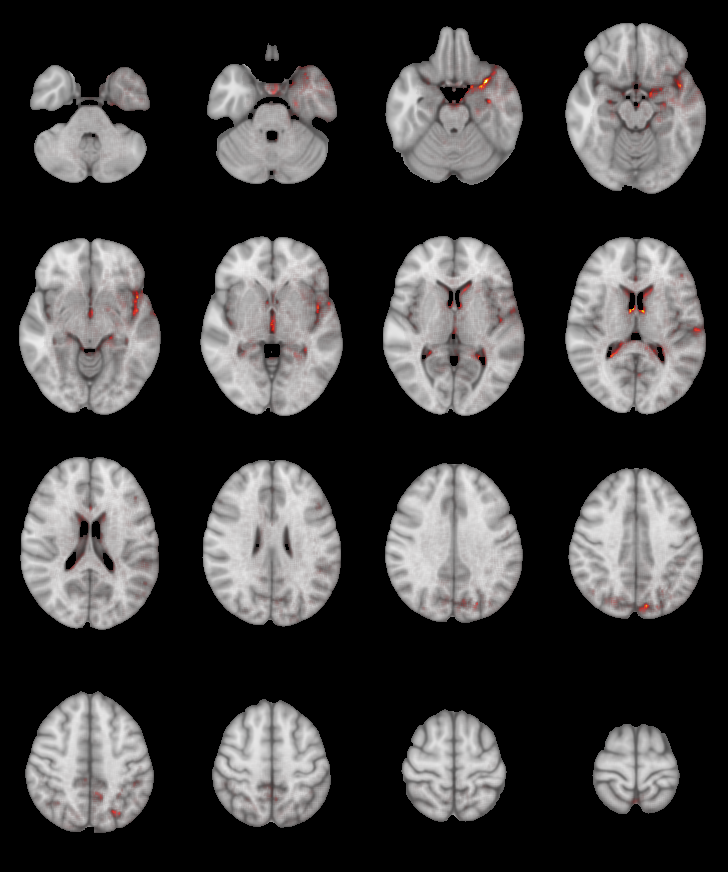
\includegraphics[width=0.31\textwidth]{data/subject1.png}
			};
			\node[anchor=north,inner sep=2pt, text=white, font=\footnotesize] at (box1.north) {Patient 1};

			\node
				[minimum height=0.41\textwidth,
				minimum width=0.32\textwidth,
				fill=black,
				anchor=west
			] (box2) at ($ (box1.east) + (0.05,0) $) {};
			\node[anchor=south] at (box2.south) {
				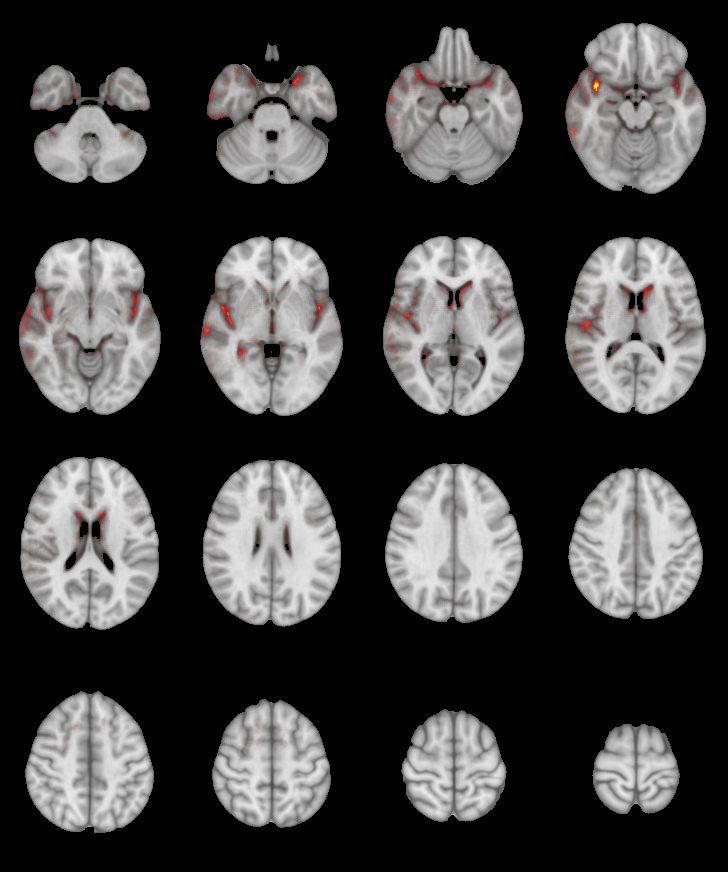
\includegraphics[width=0.31\textwidth]{data/subject2.png}
			};
			\node[anchor=north,inner sep=3pt, text=white, font=\footnotesize] at (box2.north) {Patient 2};

			\node
				[minimum height=0.41\textwidth,
				minimum width=0.32\textwidth,
				fill=black,
				anchor=west
			] (box3) at ($ (box2.east) + (0.05,0) $) {};
			\node[anchor=south] at (box3.south) {
				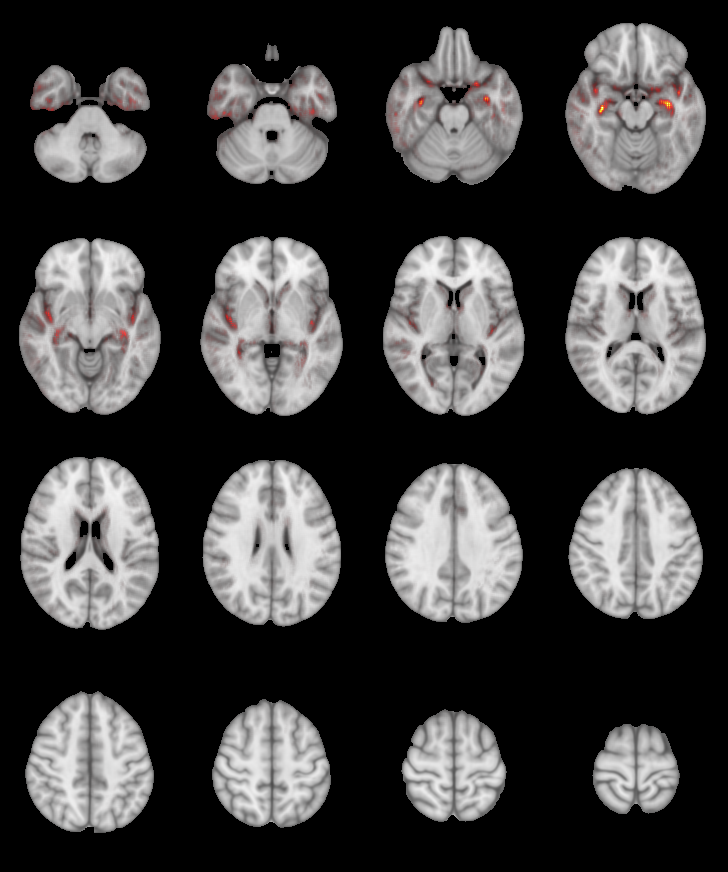
\includegraphics[width=0.31\textwidth]{data/subject3.png}
			};
			\node[anchor=north,inner sep=3pt, text=white, font=\footnotesize] at (box3.north) {Patient 3};
        }
        \visible<5>{
            \node[] at (0, 0) {
                
\includegraphics[width=5cm]{data/dementia.png}
            };
        }
        \visible<6-8>{
            \node[label={[text depth=0pt]above:Component 0}] (first) at (-3.4, 1) {
                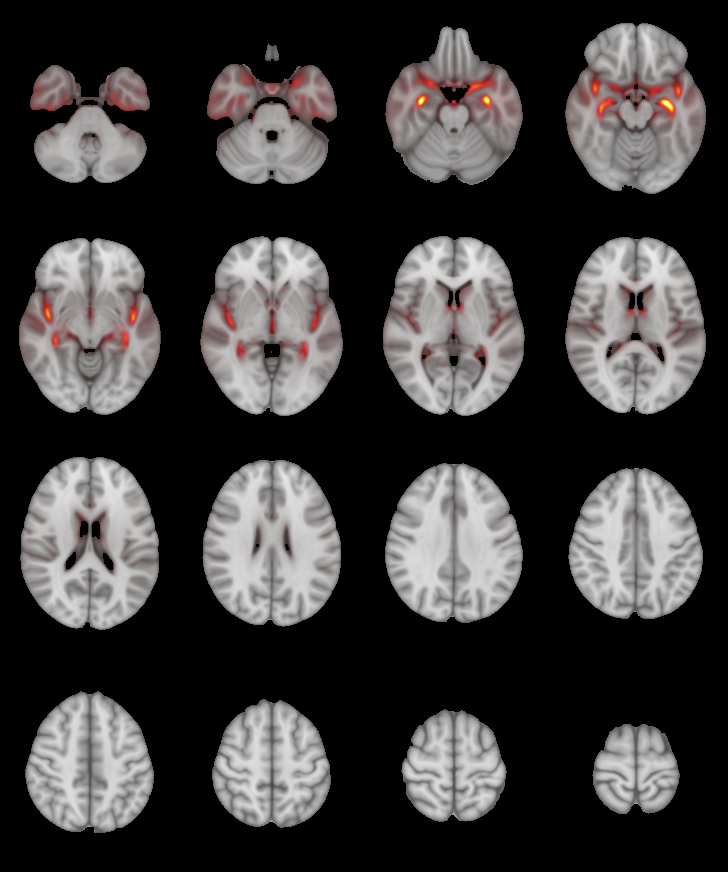
\includegraphics[
                    width=2.2cm,
                    clip=true,
                    trim = 192mm 232mm 0mm 0mm
                ]{data/components/component_0.png}
            };

            \node[anchor=west, label={[text depth=0pt]above:Component 1}] (second) at (first.east) {
                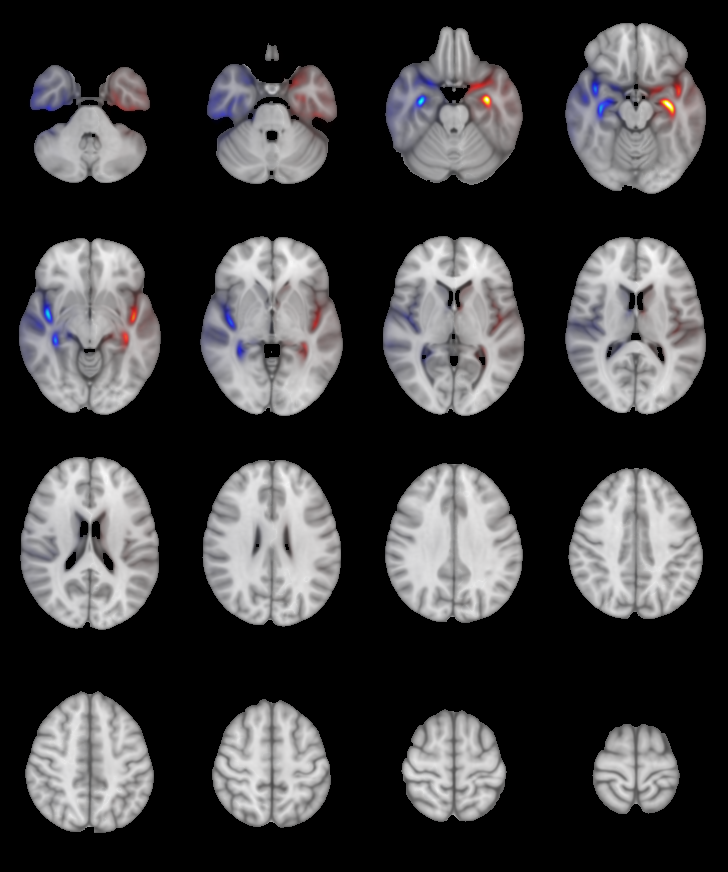
\includegraphics[
                    width=2.2cm,
                    clip=true,
                    trim = 192mm 232mm 0mm 0mm
                ]{data/components/component_1.png}
            };

            \node[anchor=west, label={[text depth=0pt]above:Component 2}] (third) at (second.east) {
                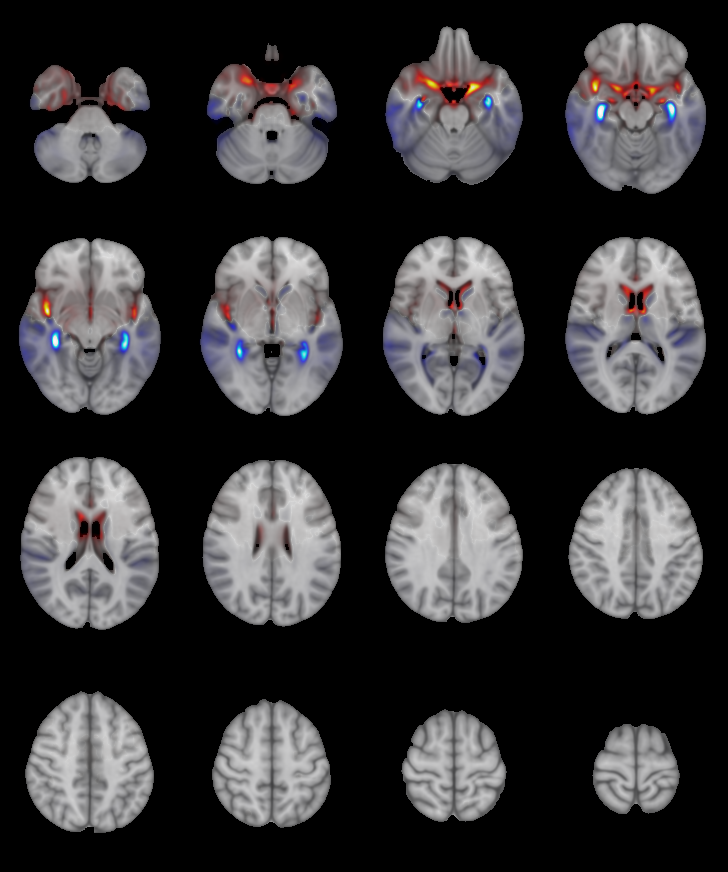
\includegraphics[
                    width=2.2cm,
                    clip=true,
                    trim = 192mm 232mm 0mm 0mm
                ]{data/components/component_2.png}
            };

            \node[anchor=west, label={[text depth=0pt]above:Component 3}] (fourth) at (third.east) {
                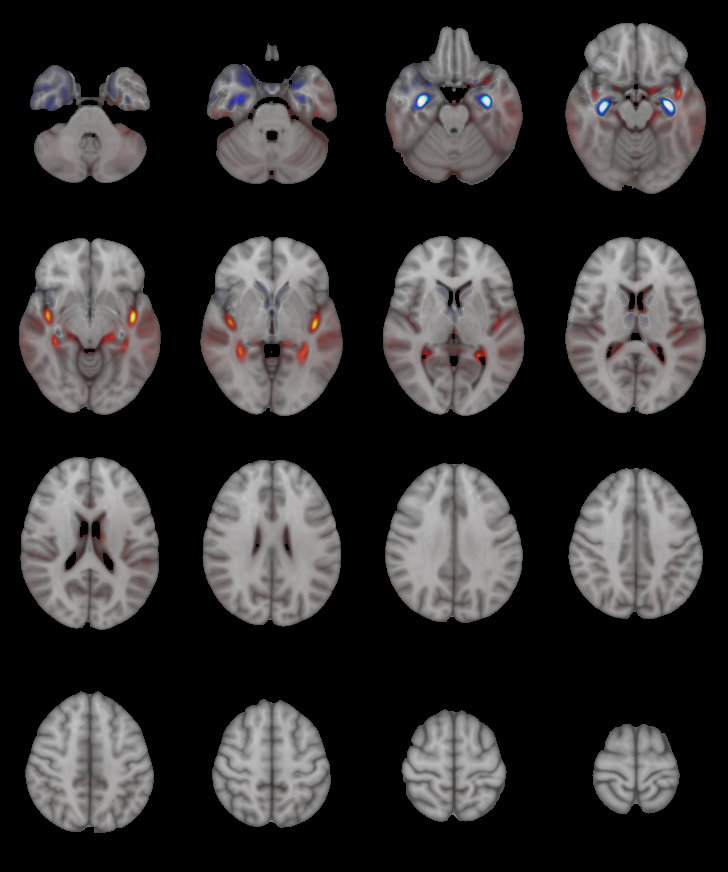
\includegraphics[
                    width=2.2cm,
                    clip=true,
                    trim = 192mm 232mm 0mm 0mm
                ]{data/components/component_3.png}
            };
        }
        \visible<7>{
            \node[anchor=north west] (first-survival) at ($ (first.south west) + (-1.17, 0.35) $) {
                \usebox{\firstsurvival}
            };
            \node[anchor=north west] (third-survival) at ($ (third.south west) + (-0.87, 0.158) $) {
                \usebox{\secondsurvival}
            };
            \node[anchor=north west] (fourth-survival) at ($ (fourth.south west) + (-0.86, 0.158) $) {
                \usebox{\thirdsurvival}
            };
            \node[anchor=north, inner sep=2pt] (legend-header) at ($ (second.south) - (0, 0) $) {\scriptsize{\underline{Percentiles}}};
            \node[anchor=north west, inner sep=1pt] (tenth) at ($ (legend-header.south east) - (0.83, 0) $) {\scriptsize{5th}};
            \node[anchor=north west, inner sep=1pt] (fiftieth) at (tenth.south west) {\scriptsize{50th}};
            \node[anchor=north west, inner sep=1pt] (ninetyeth) at (fiftieth.south west) {\scriptsize{95th}};
            \draw[draw=healthy-default, very thick, text depth=0] ($ (tenth.west) + (-0.43, 0) $) -- ($ (tenth.west) + (-0.05, 0) $);
            \draw[draw=controls-default, very thick, text depth=0] ($ (fiftieth.west) + (-0.43, 0) $) -- ($ (fiftieth.west) + (-0.05, 0) $);
            \draw[draw=cases-default, very thick, text depth=0] ($ (ninetyeth.west) + (-0.43, 0) $) -- ($ (ninetyeth.west) + (-0.05, 0) $);
        }
        \visible<8>{
            \node[anchor=north west] (first-correlation) at ($ (first.south west) + (-0.79, 0.1) $) {
                \usebox{\firstcorrelations}
            };
            \node[anchor=north west] (second-correlation) at ($ (first-correlation.north east) - (0.62, 0) $) {
                \usebox{\secondcorrelations}
            };
            \node[anchor=north west] (third-correlation) at ($ (second-correlation.north east) - (0.62, 0) $) {
                \usebox{\thirdcorrelations}
            };
            \node[anchor=north west] (fourth-correlation) at ($ (third-correlation.north east) - (0.6, -0.18) $) {
                \usebox{\fourthcorrelations}
            };
        }
    \end{tikzpicture}
\end{frame}
